\chapter{Untersuchung mit dem Lichtmikroskop und Bestimmung des Maßstabs}
Bevor das eigentliche Experiment begonnen wird, ist es unbedingt erforderlich, einen Probelauf durchzuführen, um die Eigenschaften des STM sowie alle relevanten Parameter kennenzulernen. 
Zunächst wird das Einsetzen der Spitze mit alten Spitzen geübt. Dies erfolgt, da ohne vorherige Erfahrung die neue und funktionierende Spitze sonst beschädigt werden könnte.

Die eigentliche Zerstörung der Spitze kann hauptsächlich durch mechanischen Bruch auftreten, wenn sie mit der Probe in Kontakt kommt, oder durch übermäßige Tunnelströme, wenn der Abstand zur Probe zu gering ist. 
In beiden Fällen ist ersichtlich, dass die zu erwartende Auflösung nicht erreicht werden kann; bei übermäßig hohen Strömen kann zudem Rauschen entstehen, verursacht durch das Aufschmelzen der Spitzenoberfläche. Der Spitzen-Durchmesser beträgt $\SI{0.3}{\nm}$ \cite{praktikum}. 
Die resultierenden Bilder sind in \cref{fig:Spitze} zu betrachten. 
\begin{figure}[htbp]
    \centering
    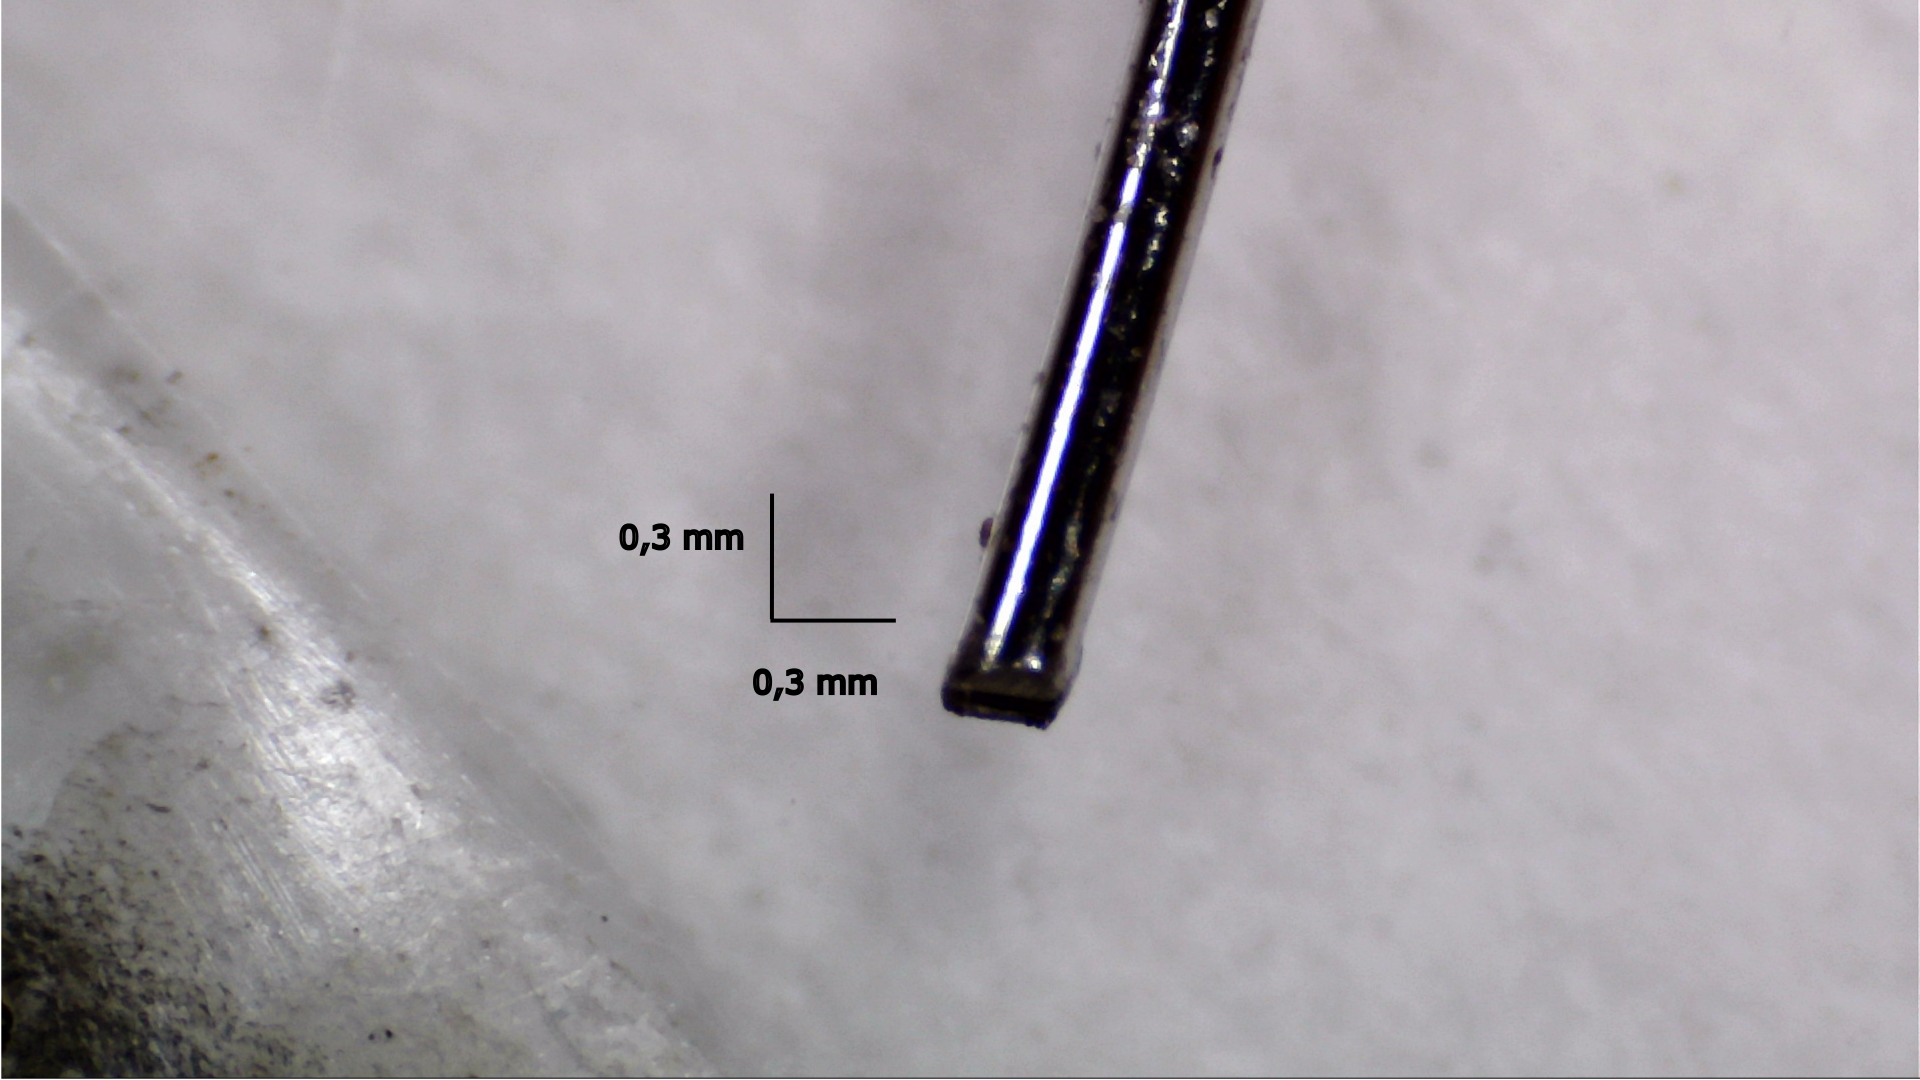
\includegraphics[width=0.75\textwidth]{editprobe_spitze.png}
    \caption{Aufnahme der Messpitze vor der Messung. Die eingezeichneten Linien entsprechen Längen von $\SI{0.3}{\mm}$.}
    \label{fig:Spitze}
\end{figure}

Da die für den Probelauf verwendete Spitze scharf abgeschnitten war, wurde sie weiterverwendet. Selbstverständlich kann nicht garantiert werden, dass die Spitze tatsächlich Einatomqualität besitzt. 
Darüber hinaus war kein signifikanter Unterschied im Zustand der Spitze vor und nach der Messung erkennbar.

Anschließend wird der Probenhalter mit Isopropanol gereinigt, um beispielsweise Hautfettrückstände zu entfernen, die aufgrund erhöhter Adhäsion durch den Piezo-Motor die Beweglichkeit beeinträchtigen könnten. 
Danach wird der wesentliche Prozess des Heranfahrens mit einem leeren, einzusetzenden Probenhalter geübt. 
Dieser Vorgang wird entweder mithilfe eines Stereomikroskops oder eines auf einem Stativ über dem STM montierten USB-Mikroskops beobachtet - in diesem Fall wurde letztere Methode gewählt. 
Wird während des Heranfahrens keine Bewegung festgestellt, sollte der Probenhalter beschwert werden, um den Kontakt zum Fahrmotor zu verbessern, und erneut gereinigt werden.\\
Es ist wichtig zu beachten, dass in diesem Stadium lediglich geprüft wird, ob der Heranfahrvorgang korrekt funktioniert - das STM selbst wird noch nicht als Abbildungsinstrument eingesetzt.
Im vorliegenden Versuchsaufbau erfolgt das Heranfahren zunächst grob über die STM-''Advance''-Funktion und wird anschließend mithilfe der ''Approach''-Funktion verfeinert. 
Im Fall der Goldprobe wird eine raue Oberflächenstruktur erwartet, weshalb der ''Constant Current Mode (CCM)'' zum Einsatz kommt. Darüber hinaus werden wolkenartige Strukturen erwartet, die die kleinen, auf das Saphirsubstrat verdampften Goldcluster repräsentieren. 
Diese Dampfabscheidung ist erforderlich, da die Probe sonst nicht leitfähig wäre.

Um im CCM-Modus zu arbeiten, werden am Controller kurze Integrationszeiten (d.h. große Werte für die I-Regelverstärkung) eingestellt, damit dieser schnell auf Änderungen des Abstands zwischen Probe und Spitze reagieren kann. Für das Heranfahren werden eine Spannung von \SI{500}{\mV} zwischen Spitze und Probe sowie ein Tunnelstrom von \SI{1}{\nA} verwendet.

Anschließend erfolgt die Kalibrierung für den Maßstab mithilfe des TEM-Gitters, das in diesem Fall mit ''$400 \times 100$'' beschriftet ist. Als Kalibrierreferenz wurde die 400-Achse verwendet. Die Bezeichnung ''$400 \times 100$'' besagt, dass diese Anzahl an Gitterquadraten in den jeweiligen Dimensionen in ein Quadratzoll passt.

Um eine Länge im Mikroskopbild zu messen, nutzt man, dass die Breite/Länge eines sichtbaren Gitterquadrats jeweils $\frac{1}{400}$ Zoll bzw. $\frac{1}{100}$ Zoll entspricht [\cite{praktikum}]. Man zählt die Anzahl der Gitterquadrate und multipliziert diese mit einem der genannten Faktoren, um die Länge des sichtbaren Abschnitts zu erhalten. Wie zuvor beschrieben dient dies nun als Maßstab, mit dem die relative Größe beobachteter Objekte im USB-Mikroskop in absolute Einheiten umgerechnet werden kann.

Das Kalibrierungsbild für das USB-Mikroskop ist in \cref{fig:Messteil} zu sehen, und das Bild der Probe ist in \cref{fig:Spitze} dargestellt.

\begin{figure}[htbp]
    \centering
    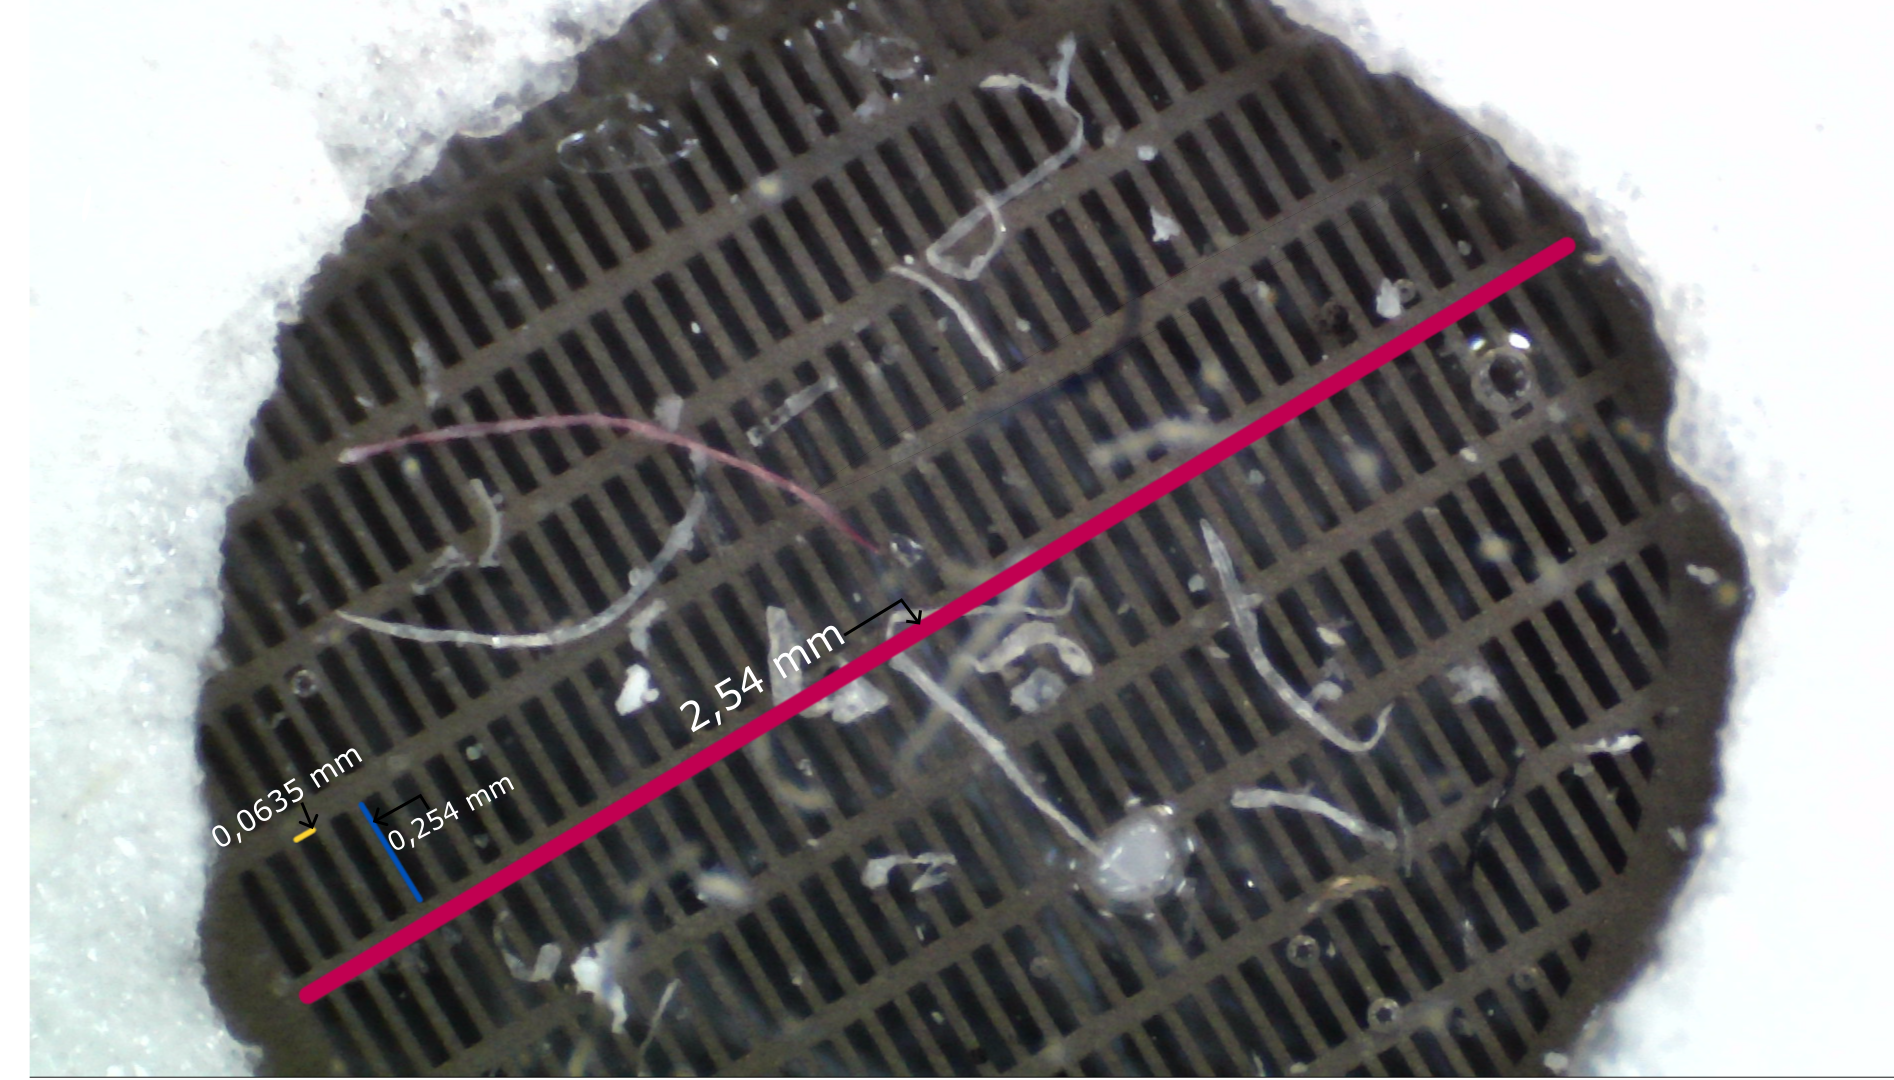
\includegraphics[width=0.75\textwidth]{edittem_messteil.png}
    \caption{Aufnahme des TEM-Netzchen mit dem USB-Mikroskop.}
    \label{fig:Messteil}
\end{figure}


